%\documentclass[normaltoc]{abnt}
\documentclass[12pt]{article}
\usepackage[utf8]{inputenc} % acentos em portugues
\usepackage[alf]{abntcite}
\usepackage{verbatim} %comentários de multiplas linhas
\usepackage[brazil]{babel}
\usepackage{graphicx}
%\hyphenrules{nohyphenation} %tirar hífens 
\hyphenpenalty = 10000
\bibliographystyle{plain}

% disables chapter, section and subsection numbering
\setcounter{secnumdepth}{-1}

\author{Bruno Farias de Loreto}

\begin{document}

\section{Instruções}

Execute main.py para executar o programa ( ./main.py ).
Você pode enviar o nome da imagem a ser processada pela linha de comando ( ./main.py simple.png ), caso
não seja passado nenhum argumento, será assumido como argumento a ``./double.png''.

Assim que o programa inicia você tem a opção de decidir se você quer usar uma imagem ou um arquivo de texto, então você pode escolher qual algoritmo usar. Após processada a imagem de treino, será mostrado o número de classificações corretas (hit) e o número de classificações incorretas (miss), e então será gerada uma imagem com 30000 pontos aleatórios. Em seguida é perguntado se você quer que o programa tente fazer uma imagem com pixels em ordem sequencial, pintando assim todos os pixels da imagem, formando uma imagem de alta qualidade, no entanto este processo pode ser lento (cerca de 1 minuto).

Note que os algoritmos podem trabalhar tanto com imagens quanto com pontos em um arquivo de texto como entrada, no entanto caso os pontos não sejam bidimensionais, o programa apenas treinará com os pontos mas não apresentará nada na tela, já que não faria muito sentido desenhar uma imagem quando cada ponto está em outras dimensões.

Adicionalmente, você também pode carregar um arquivo de texto como os de exemplo contidos neste projeto.
Estes arquivos podem descrever pontos num espaço 2D ou ND, e, nos dois casos, será escrito um arquivo de texto na pasta local chamado ``output'' que conterá os pontos classificados, com suas coordenadas e classe. No entanto note que quando os dados forem 2D, será também exibida uma imagem ilustrando o comportamento do programa. Entretanto as cores são escolhidas aleatoriamente para cada classe, portanto caso aconteça o azar da imagem ficar ruim por falta de contraste entre as classes, é recomendavél executar novamente o programa para tentar obter uma imagem com qualidade superior.

\section{Resultados e Conclusões}

Os algoritmos IBL 1 e 2 mostraram uma capacidade surpreendente visto sua simplicidade de implementação, com poucas linhas de código foi possível de se facilmente classificar uma espiral e uma espiral dupla, e com um desempenho também bastante bom.
\begin{figure}[hb]
	\center
	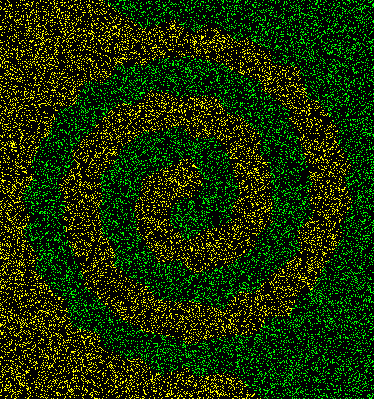
\includegraphics[width=9cm]{./outputs/double30000dots.png}
	\caption{Imagem gerada com 30000 pontos aleatórios utilizando o IBL 1.}
\end{figure}
\begin{figure}[hb]
	\center
	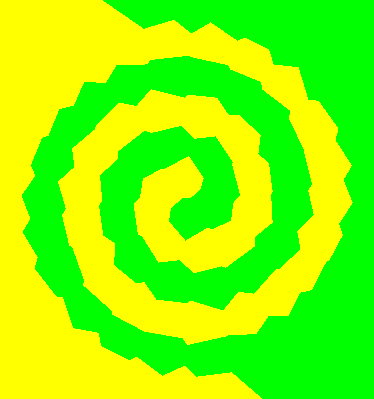
\includegraphics[width=9cm]{./outputs/sequentialdouble.png}
	\caption{Imagem gerada pintando todos os pixels da imagem utilizando o IBL 1.}
\end{figure}
Entre o IBL 1 e 2 só existe uma única linha de código diferente, e esta pequena modificação já faz mudanças profundas na maneira como é armazenado o Descritor Conceitual, tornando-o substancialmente menor, fazendo com que ele ocupe menos memória e também execute mais rápido (já que na classificação, cada ponto processado é comparado com todos do descritor conceitual). No entanto ele dá como output uma imagem um pouco mais distorcida do que o IBL 1, mas ainda gera uma imagem suficientemente boa.

\begin{figure}[hb]
	\center
	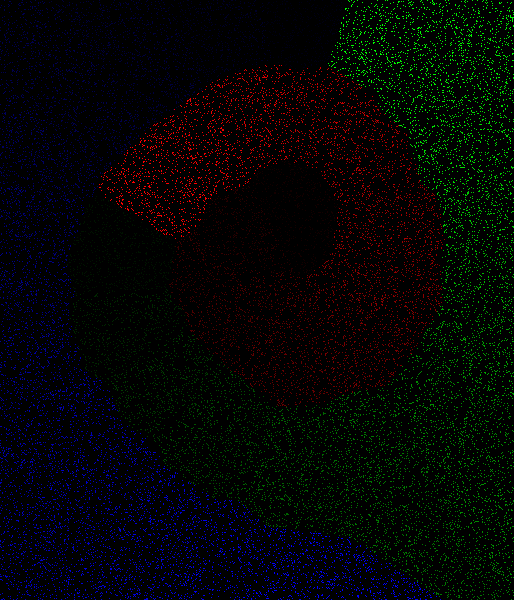
\includegraphics[width=9cm]{./outputs/simple30000dots.png}
	\caption{Imagem gerada com 30000 pontos aleatórios utilizando o IBL 2.}
\end{figure}

\begin{figure}[hb]
	\center
	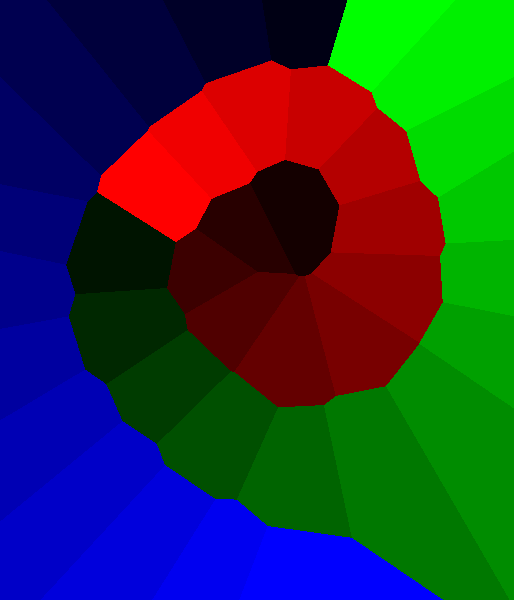
\includegraphics[width=9cm]{./outputs/sequentialsimple.png}
	\caption{Imagem gerada pintando todos os pixels da imagem utilizando o IBL 2.}
\end{figure}

Já o IBL 3 mostrou-se desafiante na sua implementação, sendo ele bem maior que suas versões anteriores. No entanto seu Descritor Conceitual pode vir a ser ainda menor do que o do IBL 2, e ainda sim ser mais consistente que o IBL 2. Isto acontece por que o IBL 3 tem um melhor critério de avaliação sobre quais pontos realmente são importantes para ser usados como classificadores e quais são ruins (tanto por já existirem vizinhos melhores tanto quando é o caso deste determinado ponto ser ruído).

Apesar do algoritmo de treino ser mais complexo, tanto na implementação, quanto no desempenho, o algoritmo de classificação ainda é o mesmo, portanto o tempo extra despendido com o treino pode compensar bastante na hora da classificação.

Fiz com que um ponto não pudesse ser eliminado do descritor conceitual sem antes ter sido usado para avaliação pelo menos 30 vezes. Isto se deve ao fato de que no começo do treinamento, a maior parte dos pontos aparenta ser um ``mal classificador'' e pontos que poderiam ser bons futuramente acabariam sendo excluídos do DC prematuramente.

\begin{figure}[hb]
	\center
	
\includegraphics[width=9cm]{./outputs/square.png}
	\caption{Imagem gerada pintando todos os pixels da imagem utilizando o IBL 3, utilizando como input o arquivo ``test.data''.}
\end{figure}

\end{document}
